%BEGIN: UbiWise 
\section{UbiWise}\label{sec:ubiwise}
\emph{UbiWise, A Simulator for Ubiquitous Computing Systems Design.}\\

UbiWise \cite{barton2003ubiwise} is a device-centric simulator. The target of this work was to allow researchers to simulate ubiquitous computing devices\footnote{networked, context-aware devices} before physical prototypes are available. The purpose of this is to empower the researcher to write software for the device and test it from a user interaction's point of view, in the actual physical environment the device was envisioned to be used in. This project emerged from two independent simulators: UbiSim and WISE.\\

To give an example of devices simulated with UbiWise, in the evaluation they have presented a wireless digital camera and wireless picture frames. The camera could easily connect to one of the frames and transfer a digital picture to be displayed.\\

UbiSim is a 3D environment simulator, aimed at producing context information in real-time, in a close to realistic environment. To simulate the environment, they have used the Quake III Arena (Q3A)\footnote{\url{http://www.idsoftware.com/gate.php}} first person shooter gaming engine, written in the C programming language. On top of the raw simulated data outputted by Q3A, they have built a \emph{context server} which processes the simulated data and delivers meaningful context data to external applications and services. The simulator is also able to process data from sensors in the real-world, generating mixed reality together with the simulated data.\\

WISE is a 2D device interaction simulator written in Java. This allows the user to interact with the software running on the device, interacting with real-world web services and other simulated devices.\\

In the 3D physical environment, the set of simulated devices are used in a context-aware manner, reacting to physical events and contextual changes. The devices might be portable, hand-held by a virtual agent the user controls (e.g. a digital camera enhanced with Internet connectivity) or they might be static devices, attached to a physical entity (e.g. a wireless enhanced picture frame on a wall). The simulation monitors the proximity between the devices, triggering events and allowing the software running on the devices to take specific actions.

In the 2D environment, the set of devices are presented in desktop-alike windows and they react to mouse clicks and network events. This allows to user to directly interact with the device through the simulated interface. Figure \ref{fig:ubiwise_2d_view} depicts a screenshot of the 2D view.\\
\begin{figure}[H]
	\centering
	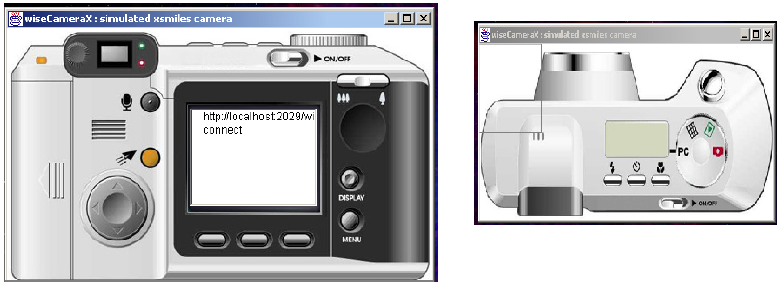
\includegraphics[width=\linewidth]{gfx/Chapter2/ubiwise_2d_view}
	\caption{UbiWise 2D view to interact with devices}
	\label{fig:ubiwise_2d_view}
\end{figure}

The simulator was developed on top of 3D game engine, empowering the agent to freely walk around the simulated environment. As the framework is device centric, the interaction between the agent and the environment is focused on interacting with the simulated devices: ''the simulator concentrates on computation and communications devices
situated within their physical environments.'' \cite{barton2003ubiwise}. One of the devices might be hand-held and carried around by the agent. There is no mention in the paper about the ability of the agent to put the hand held device down or to pick up another one. Physical objects are part of the environment, but they are not monitored and their state is not part of the system's context data. Figure \ref{fig:ubiwise_3d_view} presents a screenshot of the 3D view.\\
\begin{figure}[H]
	\centering
	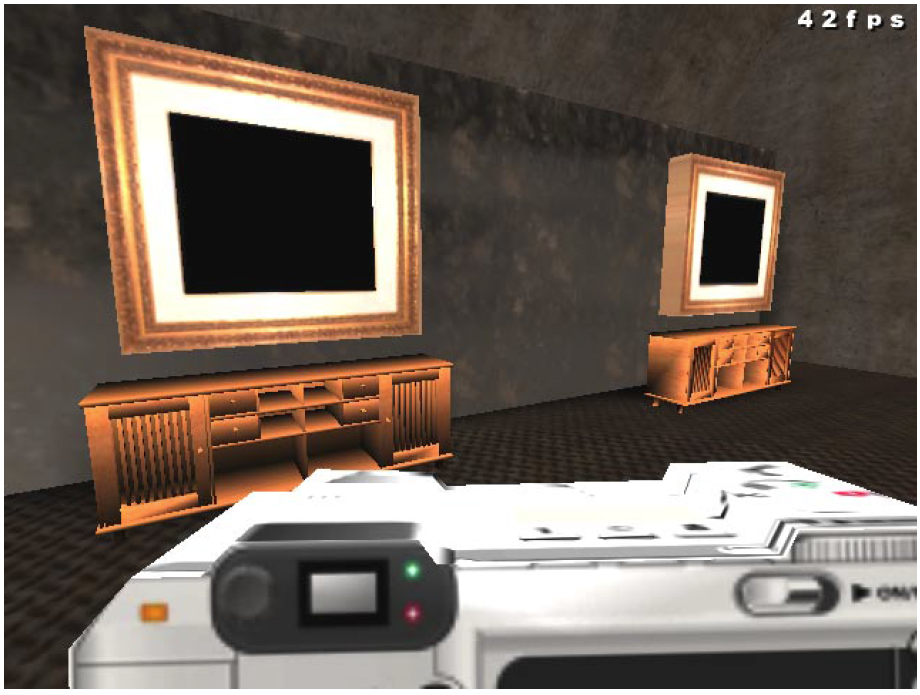
\includegraphics[width=\linewidth]{gfx/Chapter2/ubiwise_3d_view}
	\caption{UbiWise: 3D view of the physical environment}
	\label{fig:ubiwise_3d_view}
\end{figure}

UbiWise empowers the researcher to write actual software that runs on the simulated devices. The framework monitors proximity of the agent towards devices and proximity of the devices to each other, making this information available, together with other contextual data, to the software running on the devices.\\

The framework's source code is publicly available.
%END: UbiWise